% u1=(4/5,3/5), u2=(0,1), shown as free vectors based at P.
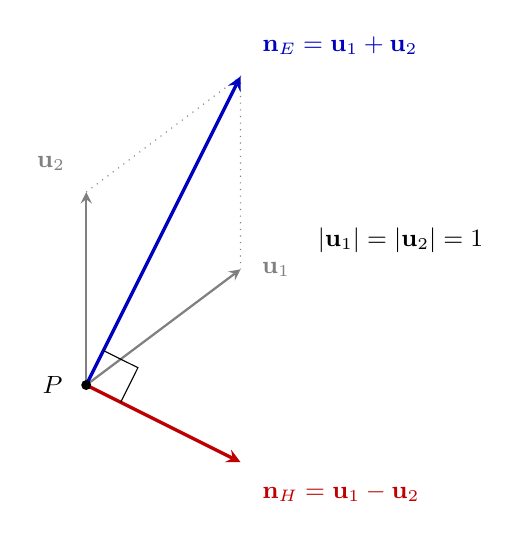
\begin{tikzpicture}[x=2.45cm,y=2.45cm,>=stealth,font=\small]
\draw[gray,dotted] (0,1)--(.8,1.6)--(.8,.6);
\draw[->,gray,thick] (0,0)--(.8,.6) node[right=4pt] {$\mathbf u_1$};
\draw[->,gray,thick] (0,0)--(0,1) node[above left=4pt] {$\mathbf u_2$};
\draw[->,blue!75!black,very thick] (0,0)--(.8,1.6)
 node[above right=4pt] {$\mathbf n_E=\mathbf u_1+\mathbf u_2$};
\draw[->,red!75!black,very thick] (0,0)--(.8,-.4)
 node[below right=4pt] {$\mathbf n_H=\mathbf u_1-\mathbf u_2$};
\draw (.089,.179)--(.268,.09)--(.179,-.089);
\fill (0,0) circle (1.8pt) node[left=5pt] {$P$};
\node[anchor=west] at (1.15,.75) {$|\mathbf u_1|=|\mathbf u_2|=1$};
\end{tikzpicture}
